\documentclass{article}

%%% SOME USEFUL PACKAGES %%%
\usepackage[english]{babel} % hyphenation
\usepackage[margin=1.5cm]{geometry} % margins
\usepackage{graphicx} % support for graphics
\usepackage{amsmath} % support for math­e­mat­i­cal typesetting
\usepackage{amssymb} % math­e­mat­i­cal symbols
\usepackage{color} % support for colors
\usepackage{mathtools} % more math­e­mat­i­cal type­set­ting
\usepackage{amsthm} % for defining theorem-like environments
\usepackage{enumerate} % change appearance of numbered lists
\usepackage{framed} % textboxes
\usepackage[format=plain,labelfont=bf,up]{caption} % cus­tomise cap­tions for fig­ures and ta­bles
\usepackage[colorlinks=true,linkcolor=black,urlcolor=blue,linktoc=all, citecolor=black]{hyperref} % hyperlinks
\usepackage{setspace}
\usepackage{verbatim}

%%% CUSTOM COMMANDS %%%
\def\ci{\perp\!\!\!\perp} % statistical independence symbol
\newcommand{\ind}{1\hspace{-2.1mm}{1}} % indicator function
\newcommand{\rl}{\mathbb{R}} % real numbers
\newcommand{\ex}[1]{\mathbb{E} \left\{ #1 \right\}} % expectation operator
\newcommand{\pr}[1]{\mathbb{P} \left\{ #1 \right\}} % probability
\newcommand{\var}[1]{\mathbb{V}\text{ar} \left\{ #1 \right\}} % variance
\newcommand{\cov}[1]{\mathbb{C}{ov} \left\{ #1 \right\}} % covariance
\newcommand{\corr}[1]{\mathbb{C}{orr} \left\{ #1 \right\}} % correlation

\begin{document}
	\title{OSM Lab 2017: Linearization Pset }
	\author{Wei Han Chia}
	\date{Due: 28 July 2017}
	\maketitle
	
	\section*{Linearization}
	
	\subsection*{Exercise 1}
	Consider the Brock and Mirman model. From the lecture notes ,we are given the following linearized form:
	\begin{align*}
	F &= \frac{\beta \alpha \bar{K}^{\alpha - 1}}{\bar{K}^{\alpha} - \bar{K}} \\
	G &= - \frac{\beta \alpha \bar{K}^{\alpha - 1} (\alpha + \bar{K}^{\alpha -1})}{\bar{K}^{\alpha} - \bar{K}}\\
	H &= \frac{\beta \alpha^2\bar{K}^{2(\alpha -1)}}{\bar{K}^{\alpha} - \bar{K}} \\
	L &= - \frac{\beta \alpha \bar{K}^{2\alpha - 1}}{\bar{K}^{\alpha} - \bar{K}} \\
	M &= \frac{\beta \alpha^2\bar{K}^{2(\alpha -1)}}{\bar{K}^{\alpha} - \bar{K}}		
	\end{align*}
	We can also substitute $\bar{K} = (\beta \alpha)^{1/(1 -\alpha)}$. Given these, we also know the values of $P$ and $Q$
	\begin{align*}
	P &= \frac{-G - \sqrt{G^2 - 4FH}}{2F}\\
	Q &= - \frac{LN+ M}{FN + FP + G}
	\end{align*}
	\begin{figure}[!h]
		\centering
		\caption{Policy Functions from Brock and Mirman Model}
		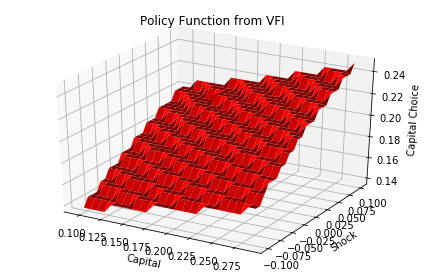
\includegraphics[scale = 0.5]{fig1}
		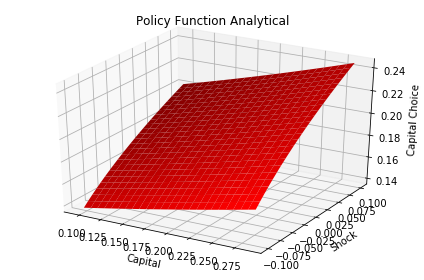
\includegraphics[scale = 0.5]{fig2}
		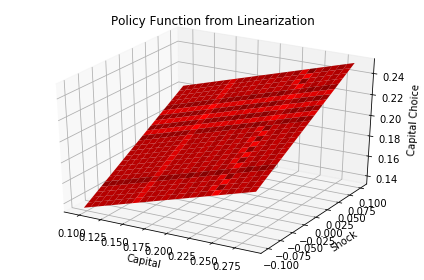
\includegraphics[scale = 0.5]{fig3}
		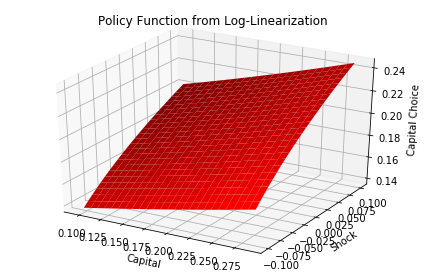
\includegraphics[scale = 0.5]{fig4}
	\end{figure}

	We can solve these values and plot the linearized policy function in python. We do this in the attached notebook. Comparing our plots with those from the previous Pset, we note that our linearized policy function provides a close approximation around the steady state, but lacks the curvature present in the other two policy functions.
	
	\subsection*{Exercise 2}
	Now if we use $k \equiv \ln K$ instead of $K$, we can substitute $K_t = e^{k_t}$ we get the following equations:
	\begin{align*}
	F &= \frac{\beta \alpha e^{\bar{k}(\alpha - 1)} e^{\bar{k}}}{e^{\bar{k} \alpha} - e^{\bar{k}}} \\
	G &= - \frac{\beta \alpha (e^{\bar{k}(2\alpha -1)} + \alpha e^{\bar{k} \alpha})}{e^{\bar{k} \alpha} - e^{\bar{k}}}\\
	H &= \frac{\beta \alpha^2 e^{\bar{k} (2\alpha -1)}}{e^{\bar{k} \alpha} - e^{\bar{k}}} \\
	L &= - \frac{\beta \alpha e^{\bar{k} \alpha}}{e^{\bar{k} \alpha} - e^{\bar{k}}} \\
	M &= \frac{\beta \alpha e^{\bar{k}(2\alpha -1)}}{e^{\bar{k} \alpha} - e^{\bar{k}}}		
	\end{align*}
	We can also substitute $\ln \bar{K} = \ln (\beta \alpha)^{1/(1 -\alpha)}$. Given these, we can find the values of $P$ and $Q$ in the same way as before.
	\begin{align*}
	P &= \frac{-G - \sqrt{G^2 - 4FH}}{2F}\\
	Q &= - \frac{LN+ M}{FN + FP + G}
	\end{align*}	
	As we can see, our log-linear policy function approximation closely matches the actual analytical solution, since that solution takes a log-linear form as well. 
	
	\subsection*{Exercise 3}
	We have the following equation
	\[ \mathbb{E}_t \left\{ F \bar{X}_{t+1} + G \bar{X}_t + H \bar{X}_{t-1} + L \bar{Z}_{t+1} + M \bar{Z}_t  \right\} = 0\]
	We can make the following substitutions
	\begin{align*}
	F \bar{X}_{t+1} &= FP \bar{X}_{t} + FQ \bar{Z}_{t+1} \\
	&= FP^2 \bar{X}_{t-1} +F PQ \bar{Z}_t + FQN \bar{Z}_t +F Q \epsilon_t \\
	G \bar{X}_t &= GP \bar{X}_t + GQ \bar{Z}_t \\
	L \bar{Z}_{t+1} &= LN \bar{Z}_{t} + L \epsilon_t
	\end{align*}
	In addition, we note that the expectation operator is linear, and $\mathbb{_t} (\epsilon_t) = 0$. To get
	\begin{align*}
	[(FP + G)P + H]\bar{X}_{t-1} + [(FQ + L)N + (FP + G)Q + M] \bar{Z}_t = 0
	\end{align*}
	
	\subsection*{Exercise 4}
	We set-up and solve the baseline tax model with the following assumptions on utility functions and production functions.
	\begin{align*}
	u(c_t, l_t) &= \frac{c_t^{1-\gamma} - 1}{1 - \gamma} + a \frac{(1 -l_t)^{1 - \xi} -1}{1 -\xi} \\
	F(K_t, L_t, z_t) &= K_t^{\alpha}(L_t e^{z_t})^{1-\alpha} 
	\end{align*}
	This yields the following Euler Equations characterizing the dynamics of the problem:
	\begin{align*}
	c_t^{-\gamma} &= \beta \mathbb{E}_t \left\{ c_{t+1}^{-\gamma}[(r_{t+1} - \delta)(1-\tau) - 1]\right\} \\
	w(1-\tau)c_t^{-\gamma} &= a(1-L)^{-\xi} 
    \end{align*}
    
    This problem is analogous to the one we solved in exercise 6 in the previous problem set, and so we check that all the steady state values given our parameters ($\gamma = 2.5, \xi = 1.5, \beta = .98, \alpha = .40, a = .5, \delta = .10, \bar{z} = 0, \rho_z = .9, \tau = .05$) are the same.
    \begin{figure}[!h]
    	\centering
    	\caption{Steady State Values from Baseline Taxation Model}
    	\begin{tabular}{c | c}
    		Variable & Steady State Value\\
    		\hline
    		k = K & 4.225\\
    		l = L& 0.579\\
    		w = W & 1.328 \\
    		r = R & 0.121 \\
    		T & 0.004 \\
    		C & 0.818 \\
    		I & 0.423 \\
    		Y & 1.28  \\
    		\hline
    	\end{tabular}
    \end{figure}
    
    In order to use this model for the subsequent questions, we recode the Euler Equations and other characterizing equations into functions. This implementation can be found in the attached python notebook.
    
    \subsection*{Exercise 5}
    We numerically compute this matrix of partial derivatives in python using centered differences. The matrix is arrayed as follows:
    \begin{align*}
    \frac{\partial y}{\partial x} &= \begin{bmatrix} \frac{\partial y_j}{\partial x_i}\end{bmatrix}
    \end{align*}
    Where $y_j = \{ K, L, w, r, T, c, y, i \}$ and $x_i = \{ \alpha, \beta, \gamma, \xi, \tau, \delta, a, \bar{z} \}$
    
    \subsection*{Exercise 6}
    We can solve the model dynamics using the provided linapp code. Here, we let $X_t = K_{t}$ be the endogenous state variable, and $Y_t = l_t$ be the endogenous choice variable. We solve this in the attached python notebook, and obtain values of 
    \begin{figure}[!h]
    	\centering
    	\caption{Uhlig Matrices from Baseline Taxation Model}
    	\begin{tabular}{c | c}
    		Matrix & Value \\
    		\hline
    		F & -2.904 \\
    		G & 5.888 \\
    		H & -2.967 \\
    		L & 2.168 \\
    		M & -2.236 \\
    		N & 0.95 \\
    		P & 0.915 \\
    		Q & 0.438 \\
    		\hline
    	\end{tabular}
    \end{figure}
    
    \newpage
    \subsection*{Exercise 7}
    Next, we can simulate 10.000 artificial time series of 250 period long economies. We start each simulation at $k = \arccos{k} = 4.225$, and $z = 0$. We also note that given the matrices P and Q, we can find $\tilde{K}_t = P \tilde{K}_{t-1} + Q \tilde{Z}_{t}$ and $\tilde{L}_t = R \tilde{K}_{t-1} + S \tilde{Z}_t$. Then, with the sequence of $\tilde{K}, \tilde{L}, \tilde{Z}$, we can back out $K_t = \bar{K} e^{\tilde{K}_t}$, $L_t = \bar{L} e^{\tilde{L}_t}$, and $Z_t = \tilde{Z}_t - \bar{Z}$. 
    
    \begin{figure}[!h]
    	\centering
    	\caption{Model Simulations for Baseline Taxation Model}
    	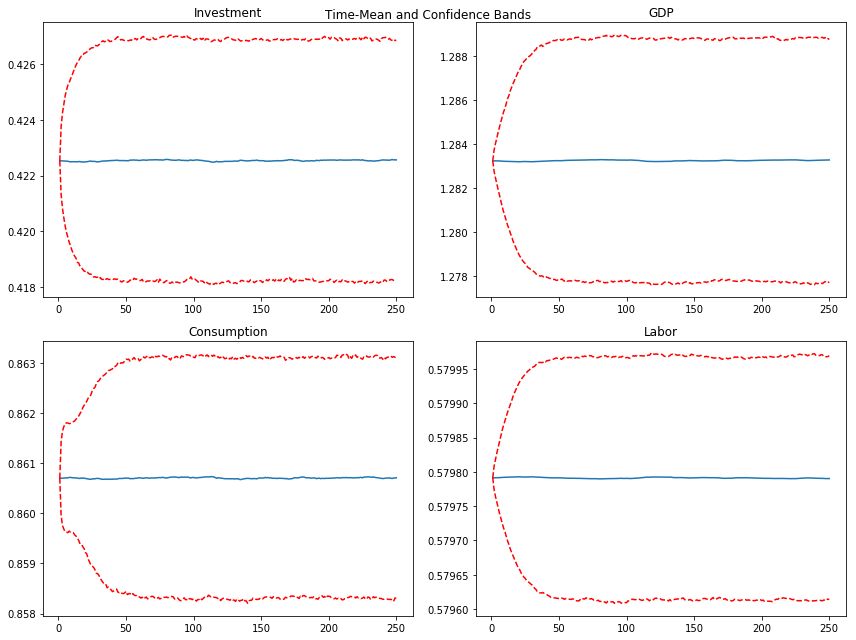
\includegraphics[scale = 0.5]{fig5}
    \end{figure}
    
    As we would expect, the time mean hovers around a fixed point. However, we also note that the confidence bands increase as we simulate the model, since the variation from the shocks increases as we increase time.
    
    \subsection*{Exercise 8}
    With the same results, we can also calculate the mean, volatility, coefficient of variation, relative volatility, persistence and cyclicality of each series over each simulation. We report these values as the mean and standard errors of these moments over the 10000 simulations.
    
    \begin{figure}[!h]
    	\centering
    	\caption{Model Moments From Simulation}
    	\begin{tabular}{c | c  c c  c}
    		Moment & GDP & Consumption & Investment & Labor \\
    		\hline
    		Mean & 1.283 & 0.861 & 0.423 & 0.579 \\
    		& (0.00152) & (0.000493) & (0.00103)& (4.84e-5) \\
    		Volatility & 0.00276 & 0.00128 & 0.00232& 8.87e-5 \\
    		& (0.000726) & (0.000224) & (0.000459) &  (2.32e-5)\\
    		Coefficient of Variation & 497.9 & 691.845 & 189.3 & 7001.7 \\
    		& (136.2) & (119.5) & (37.17)&  (1899) \\
    		Relative Volatility & 1 & 0.476 & 0.855 & 0.0321 \\
    		& (0) & (0.0580) & (0.0726) & (8.90e-5) \\
    		Persistence & 0.992 & 0.921 & 0.942& 0.990\\
    		& (0.0044) & (0.0273) & (0.0228) & (0.00502)\\
    		Cyclicality & 1 & 0.533 & 0.883 & -0.999\\
    		& 8e-17 & (0.129) & (0.0321) & (0.000115) \\
    		\hline
    	\end{tabular}
    \end{figure}
    
    \subsection*{Exercise 9}
    Finally, we can also generate impulse response functions. We code this up in the attached python notebook, and showcase a plot for $1.1 \bar{K}$. 
    
    \begin{figure}[!h]
    	\centering
    	\caption{Impulse Response from Baseline Taxation Model}
    	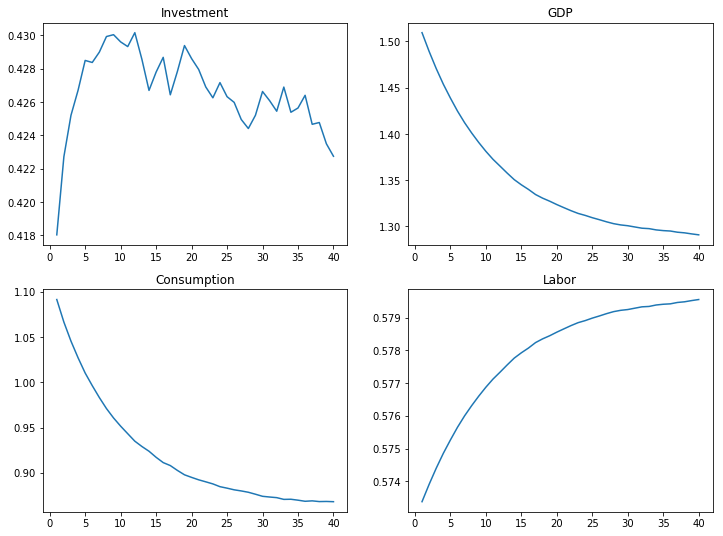
\includegraphics[scale = 0.5]{fig6}
    \end{figure}
    
    \subsection*{Exercise 10}
    In the OLG model with no labor supply, we note that given capital stocks for each group, we can back out the interest rate and wage rate from the firm FOC's, and the household consumption from the household budget constraint. 
    
    Therefore, we note that we can define $\Gamma(K_{t+2}, K_{t+1}, K_t, Z_{t+1}, Z_t)$ as the vector function yielding
    \begin{align*}
    \Gamma_1 = c_{1,t}^{-\sigma} /(\beta c_{2,t+1}^{-\sigma} (1 - r_{t+1} - \delta)) - 1
    \Gamma_2 = c_{2,t}^{-\sigma} /(\beta c_{3,t+1}^{-\sigma} (1 - r_{t+1} - \delta)) - 1
    \end{align*}
    We present the solution to the OLG model in the attached python notebook. We conclude that the accuracy of TPI is superior, but it also takes a longer time to compute compared to our linearization methods. 
    
    \begin{figure}[!h]
    	\centering
    	\caption{Comparison of Time Paths for TPI and Linearization}
    	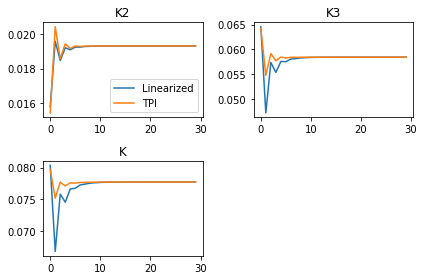
\includegraphics[scale = 0.5]{fig7}
    \end{figure}
    
    \newpage
    \subsection*{Exercise 11}
    Given the code from Exercise 10, we can easily simulate our model to replicate the same path and confidence bands given a stochastic shock.
    
    \begin{figure}[!h]
    	\centering
    	\caption{Time Series and Confidence Bands from OLG Model}
    	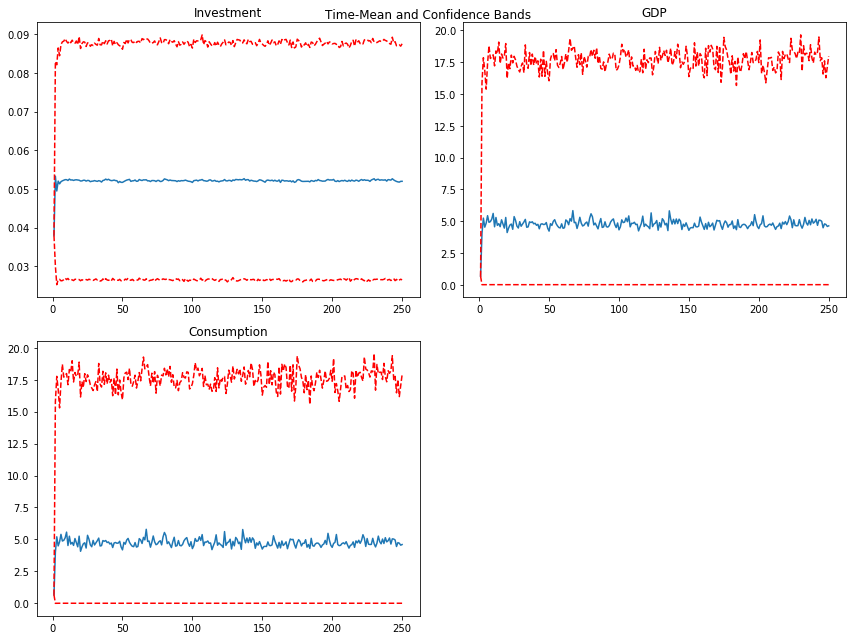
\includegraphics[scale = 0.5]{fig8}
    \end{figure}
 
\end{document}